%
% teil3.tex -- Beispiel-File für Teil 3
%
% (c) 2020 Prof Dr Andreas Müller, Hochschule Rapperswil
%
% !TEX root = ../../buch.tex
% !TEX encoding = UTF-8
%
\subsection{Mutation
\label{buch:paper:varalg:subsection:mutation}}
\rhead{Mutation}
Dieser Schritt sorgt dafür, dass zufällige Änderungen in 
den Genen stattfinden. Dadurch entstehen neue Variationen, welche
in der Kreuzung nicht entstanden wären und er vergrössert den 
gesamten Lösungsraum. Zusätzlich soll es verhindern,
dass nach einer Anzahl von Generationen immer wieder die
gleichen Genmuster entstehen, wodurch verhindert werden soll, dass 
der Algorithmus in einem lokalen Extrempunkt stecken bleibt. 
Die Mutation findet auch nicht bei jedem Kind
statt, sondern wie in der Natur werden diese per Zufall
ausgelöst. Die Mutation läuft so ab, dass über den String
iteriert wird. Auf jeder Position wird gewürfelt. Ist 
die Bedingung im Zusammenhang mit der gewürfelten Zahl erfüllt, dann wird 
die Stelle invertiert, wie in der
Abbildung \ref{fig:mutation_genetic_string} dargestellt.
\begin{figure}
	\centering
	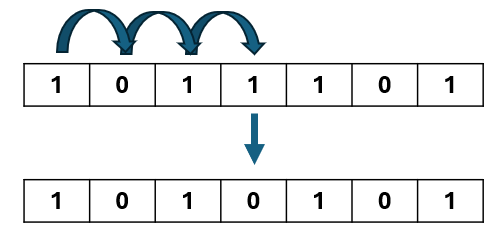
\includegraphics[width=0.8\textwidth]{
        papers/varalg/images/teil3/09GeneticStringMutation.png
        }
	\caption{
	Beispiel einer Mutation mit einem genetischen String aus 0 und 1. Die
	Mutation wird zufällig ausgelöst und invertiert die Stelle.
	}
	\label{fig:mutation_genetic_string}
\end{figure}

\subsection{Mutation auf das TSP angepasst
\label{buch:paper:varalg:subsection:mutation_tsp}}
\rhead{Mutation TSP}
Für das Travelling Salesman Problem wird die Mutation so angepasst,
dass, wenn eine Mutation stattfindet, zwei zufällige Stellen ausgewählt
werden und diese Städte werden vertauscht, 
wie in der Abbildung \ref{fig:mutation_genetic_string_cities}.
\begin{figure}
	\centering
	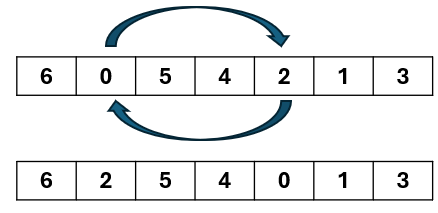
\includegraphics[width=0.8\textwidth]{
        papers/varalg/images/teil3/09GeneticStringCitiesMutation.png
        }
	\caption{Beispiel einer Mutation mit Städten}
	\label{fig:mutation_genetic_string_cities}
\end{figure}
